\section{Základní parametry zemského elipsoidu} \label{appRefEll}

\begin{table}[ht!]
\begin{tabular}{c l}

a & hlavní poloosa meridiánové elipsy \\
b & vedlejší poloosa meridiánové elipsy\\
f & zploštění (první)\\
n & zploštění (druhé)\\
e & excentricita (první)\\
$e^{'}$ & excentricita (druhá)\\
c & pólový poloměr křivosti\\
M & meridiánový poloměr křivosti\\
N & příčný poloměr křivosti\\
R & střední poloměr křivosti\\
r & poloměr rovnoběžky\\
$\varphi$ & zeměpisná šířka\\
$B_{0}^{\varphi}$ & délka oblouku meridiánu od rovníku po $\varphi$ \\
W & první geodetická funkce\\
V & druhá geodetická funkce\\
F & pomocná geodetická funce\\      
\end{tabular}
\end{table}

\begin{equation}
f = (a-b)/a.
\end{equation}

\begin{equation}
n = (a-b)/(a+b).
\end{equation}

\begin{equation}
e^{2} = (a^{2}-b^{2})/a^{2}.
\end{equation}

\begin{equation}
e^{'2} = (a^{2}-b^{2})/b^{2}.
\end{equation}

\begin{equation}
c = a^{2}/b.
\end{equation}

\begin{equation}
M = a\left(1-e^{2}\right) / W^{3}.
\end{equation}

\begin{equation}
N = a/W.
\end{equation}

\begin{equation}
R = \sqrt{M N}
\end{equation}

\begin{equation}
r = N\cos{\left(\varphi\right)}.
\end{equation}

\begin{equation}
W = \sqrt{1-e^{2}\sin^{2}{\left(\varphi\right)}}
\end{equation}

\begin{equation}
V = \sqrt{1+e^{'2}\cos^{2}{\left(\varphi\right)}}
\end{equation}

\begin{equation}
F = \sqrt{1+n\cos{\left(2\varphi\right)}+n^{2}}
\end{equation}

\section{Konstanty základních referenčních elipsoidů} \label{appRefEllConst}

\subsection{World Geodetic System 1984 (WGS84)}\label{appRefEllConstWGS84}
\begin{table}[ht!]
\begin{tabular}{c c c}
$a = 6 378 137 m$ & $b = 6 356 752,31425 m$ & $f = 0,00335 28106 64747$ \\
\end{tabular}
\end{table}

\subsection{Geodetic Reference System 1980 (GRS80)}
\begin{table}[ht!]
\begin{tabular}{c c c}
$a = 6 378 137 m$ & $b = 6 356 752,31414 m$ & $f = 0,00335 28106 81182$ \\
\end{tabular}
\end{table}

\subsection{Konstanty Krasovského elipsoidu}
\begin{table}[ht!]
\begin{tabular}{c c c}
$a = 6 378 245 m$ & $b = 6 356 863,01877 m$ & $f = 0,00335 23298 69259$ \\
\end{tabular}
\end{table}


\section{Pseudokódy implementovaných transformácii v Matlab package +Geo}

\subsection{ECEF2ENU} \label{appEcef2Enu}

\begin{algorithm}[H]
 \KwData{x, y, z, $\varphi$, $\lambda$, hel, RT, ELL}
 \KwResult{e, n, u}
 výpočet rotační matice $\mathbf{R}\left(\varphi, \lambda\right)$\;	
 \eIf{RT == elipsoid}{
  $[x_{0}, y_{0}, z_{0}] = geod2ecef(\varphi, \lambda, hel, ELL)$\;
  }{
  $[x_{0}, y_{0}, z_{0}] = sphere2ecef(\varphi, \lambda, hel^{*})$\;
 }
 Výpočet podle rovnice \ref{rov:ecef2enu22}
 \caption{Transformácia ECEF2ENU}
\end{algorithm} 

\subsection{ENU2ECEF} \label{appEnu2Ecef}

\begin{algorithm}[H]
 \KwData{e, n, u, $\varphi$, $\lambda$, hel, RT, ELL}
 \KwResult{x, y, z}
 výpočet rotační matice $\mathbf{R}\left(\varphi, \lambda\right)$\;	
 \eIf{RT == elipsoid}{
  $[x_{0}, y_{0}, z_{0}] = geod2ecef(\varphi, \lambda, hel, ELL)$\;
  }{
  $[x_{0}, y_{0}, z_{0}] = sphere2ecef(\varphi, \lambda, hel^{*})$\;
 }
 Výpočet podle rovnice \ref{rov:ecef2enu33}
 \caption{Transformácia ENU2ECEF}
\end{algorithm} 

\subsection{GEOD2ECEF} \label{appGeod2Ecef}

\begin{algorithm}[H]
 \KwData{$\varphi$, $\lambda$, h, ELL}
 \KwResult{x, y, z}
 výpočet potřebních parametrů rotačního elipsoidu (a, b, N)
 
 Výpočet podle rovnice \ref{rov:geodEcef}
 \caption{Transformácia GEOD2ECEF}
\end{algorithm} 

\subsection{ECEF2GEOD} \label{appEcef2Geod}

\begin{algorithm}[H]
 \KwData{x, y, z, ELL}
 \KwResult{$\varphi$, $\lambda$, h}
 výpočet potřebních parametrů rotačního elipsoidu (například a, e)
 
 Výpočet podle algoritmu diskutovaný např. \cite{Vermeille2011}.
 \caption{Transformácia ECEF2GEOD}
\end{algorithm} 

\section{Smerové kosíny}

\section{Elipsa chýb a Helmertová krivka}

K určeniu presnosti dvojrozmernej náhodnej veličiny je vhodné správne rozumieť chybám v rovine. Presnosť je po štatistickej stránke daná dvoma odchýlkami s normálnym rozdelením. Presnosť je teda v konkrétnom súradnom systéme, napr. v systéme pravouhlých kartézianských súradníc x, y, definovaná tzv. kovariančnou maticou v tvare:

\begin{equation}\label{rov:el1}
\mathbf{Q}=
\begin{pmatrix} 
\sigma_x             & \sigma_{x}\sigma_{y}  \\  
\sigma_{x}\sigma_{y} & \sigma_{y} 
\end{pmatrix}, 
\end{equation}

kde 

\begin{itemize}
\item $\sigma_{x}$ je druhá odmocnina rozptylu veličiny x a reprezentuje charakteristiku presnosti tejto veličiny,
\item $\sigma_{y}$ je druhá odmocnina rozptylu veličiny y a rovnako reprezentuje charakteristiku presnosti tejto veličiny,
\item $\sigma_{x}\sigma_{y}$ je kovariancia medzi parametrami x a y (v literatúre $\sigma_{x, y}$ alebo $Cov_{x, y}$).
\end{itemize}
  
Plochu elipsy, ktorú odvodíme z informácií z danej kovariančnej matice \ref{rov:el1}, opisujú tri základné veličiny: a) smerodajná odchýlka v smere hlavnej polosi $\sigma_a$, b) smerodajná odchýlka v smere vedľajšej poloosi $\sigma_b$ a c) uhol natočenia celej plochy $\vartheta$. Tieto kolmé smerodajné odchýlky spoločne s uhlom natočenia je možné odvodiť viacerými spôsobmi. Sledujúc prácu \cite{Hampacher2003}, vychádzajme z predpokladu, že hustota pravdepodobnosti je definovaná predpisom:

\begin{equation}
\varphi(x, y) = \dfrac{1}{2 \pi \sigma_{x} \sigma_{y} \sqrt{(1-\rho^2)} }  \exp\left\lbrace \dfrac{-1}{2 \left( 1- \rho^2 \right)} \left[ \frac{x^2}{\sigma_{x}^{2}} + \frac{y^2}{\sigma_{y}^{2}} -2 \rho \frac{xy}{\sigma_{x} \sigma_{y}} \right] \right\rbrace,
\end{equation}
kde

\begin{itemize}
\item  $\rho$ je koeficient korelácie.
\end{itemize}
V prípade, ak veličiny x a y sú nezávislé, koeficient korelácie je nulový. Naopak, ak veličiny sú korelované dostaneme rovnicu elipsy v tvare:

\begin{equation}\label{rov:oko}
 \dfrac{1}{1-\rho^2} \left( \dfrac{x^2}{\sigma_{x}^{2}} + \dfrac{y^2}{\sigma_{y}^{2}} -2 \rho \frac{xy}{\sigma_{x} \sigma_{y}} \right)  = t^2,
\end{equation}
kde \textit{t} je normovaná veľkosť dvojrozmernej chyby.

Ďalej bez ďalšieho odvodenia, dôjdeme k výsledku, podľa ktorého veľkosť hlavnej osi elipsy (smerodajnej odchýlky $\sigma_a$) je:

\begin{equation}\label{rov:sigA}
\sigma_a = \left\lbrace \dfrac{1}{2} \left[ \sigma_x^2 + \sigma_y^2 + \sqrt{\left(\sigma_{x}^{2}-\sigma_{y}^{2}\right)^2 + 4\rho\sigma_{x}^2\sigma_{y}^2} \right]\right\rbrace^{\dfrac{1}{2}},
\end{equation}
a veľkosť vedľajšej osi elipsy
\begin{equation}\label{rov:sigB}
\sigma_b = \left\lbrace \dfrac{1}{2} \left[ \sigma_x^2 + \sigma_y^2 - \sqrt{\left(\sigma_{x}^{2}-\sigma_{y}^{2}\right)^2 + 4\rho\sigma_{x}^2\sigma_{y}^2} \right]\right\rbrace^{\dfrac{1}{2}}.
\end{equation}

Natočenie elipsy môžeme opísať vzorcom

\begin{equation}\label{rov:nat}
\tan{\left(2\vartheta\right)} = 2\rho\dfrac{\sigma_{x}\sigma_{y}}{\sigma_{x}^2 - \sigma_{y}^2}.
\end{equation}

K rovnakému výsledku sa dá dôjsť spektrálnym rozkladom kovariančnej matice $\mathbf{Q}$ (náčrt rozkladu a odvodenia je v prílohe).

Význam veličín $\sigma_a$, $\sigma_b$ a $\vartheta$ sa často zobrazuje ako elipsa chýb a je to krivka, ktorá spojuje body s rovnakou hustotou pravdepodobnosti. To znamená, že hlavná poloosa, ktorá je odvodená od rovnice \ref{rov:sigA} je od pôvodnej súradnej sústavy odklonená o uhol opísaný rovnicou \ref{rov:nat} a že rovnica \ref{rov:oko} obecne definuje okolie skutočnej polohy veličiny, v ktorom by sa teoreticky malo vyskytovať isté percento možných hodnôt.

Z uvedeného rozloženia chýb v rovine je možné, opäť s istou pravdepodobnosťou, odvodiť aj neistotu určenia polohy bodu v ľubovoľnom smere. Krivka, ktorá spojuje presnosť pre všetky smery sa nazýva \textit{Helmertová krivka}.

Pre odhad presnosti použijeme zákon hromadenia stredných chýb. Všeobecný zápis zákona je tento \cite{Hampacher2003}:

\begin{equation}
m_f^2 = \mathbf{f}^T\mathbf{Q}\mathbf{f},
\end{equation}
kde
\begin{itemize}
\item $\mathbf{f}$ je vektor smerových kosínov,
\item $\mathbf{Q}$ je hore definovaná kovariančná matica a
\item $m_f^2$ je prievodič bodu Helmertovej krivky, t.j. veľkosť rozptylu v smere danej priamky $\sqrt{x^2+y^2}$.
\end{itemize}

Bez odvodenia, rovnica Helmertovej krivky je %\cite{Kocandrlova2000}, \cite{Hampacher2003}.

%[Hampacher2003] Hampacher M., (2003). Elipsa chyb a Helmertova křivka trochu jinak. Geodetický a kartografický obzor, 49/91, číslo 10.
%[Kocandrlova2000] Kočandrlova M., (2000). Helmertová křivka. Geodetický a kartografický obzor 46/88, číslo 6.

Jej vyjadrenie je
\begin{equation}
 \left( x^2 + y^2\right)^2 = x^2\sigma_x^2 + y^2\sigma_y^2 + 2\rho \sigma_x \sigma_y xy.
\end{equation}

\newpage
\subsection{Príklad zobrazenia elipsy chýb a Helmertovej krivky}

Prvý príklad poukazuje na stav v ktorom kovariančná matica vyjadruje nezávislé veličiny.

Jej vyjadrenie je: 

\begin{equation}
\mathbf{Q}=
\begin{pmatrix}
 2 & 0  \\
 0 & 5
\end{pmatrix}.
\end{equation}

\begin{figure}[ht!]
\begin{center}
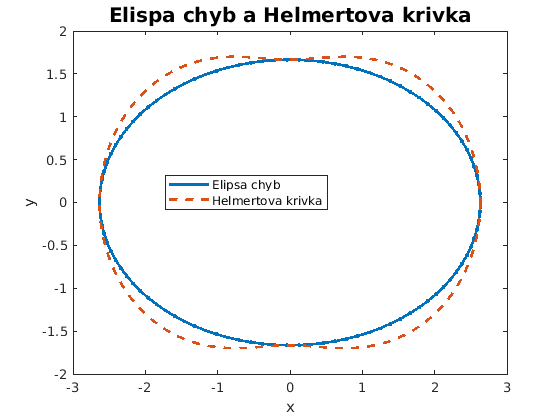
\includegraphics[width=0.5\textwidth]{FIG/s2-5cov0-0.png}
\end{center}
\caption{Zobrazenie elipsy chýb a Helmertovej krivky. Kovariancia je 0.0.}
\end{figure}

Druhý príklad poukazuje na stav v ktorom kovariančná matica vyjadruje závislé veličiny.

Jej vyjadrenie je: 

\begin{equation}
\mathbf{Q}=
\begin{pmatrix} 
  2 & 1.5  \\
1.5 & 5 
\end{pmatrix}.
\end{equation}

\begin{figure}[ht!]
\begin{center}
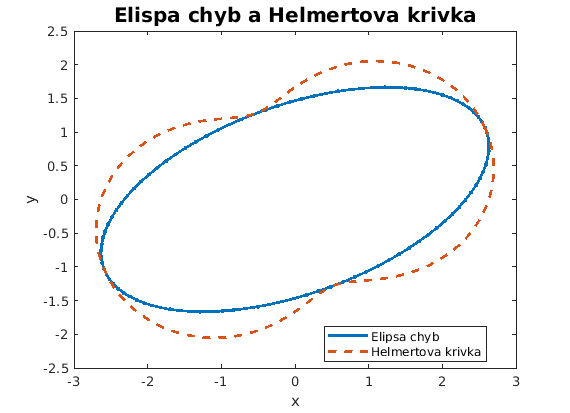
\includegraphics[width=0.5\textwidth]{FIG/s2-5cov1.5-1.5.png}
\end{center}
\caption{Zobrazenie elipsy chýb a Helmertovej krivky. Kovariancia je 1.5.}
\end{figure}

Posledný príklad obshahuje stav transformácie kovariančnej matice zo systému ECEF do systému ENU pravouhlých súradníc. Scatter ploty pod diagonálou obsahujú aj porovnanie elíps chýb a Helmertových kriviek. Z príkladu je pozorovateľné, že ak sa druhé odmocniny rozptylov veličín približne rovnajú a veličiny nie sú korelované (v príklade takými veličinami sú súradnice N (north) a U (up) v korelácii so súradnicou E (east)) tak polygóny elipsy chýb a Helmertových kriviek sa veľmi zhodujú. Naopak, ak sú data korelované (z príkladu pozorujeme závislosť veličín N a U), vidíme neistoty určenia polôh bodov v danom smere značne odlišné (bola uvažovaná $90\%$ hladina významnosti).

\begin{figure}
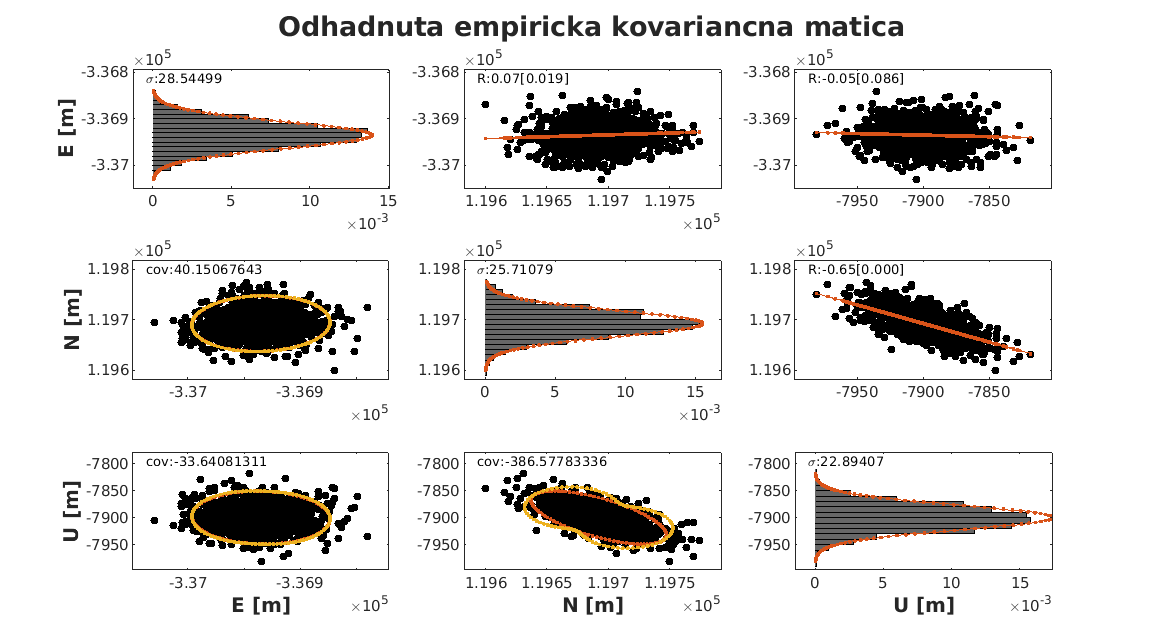
\includegraphics[width=1.0\textwidth]{FIG/ecef2enu.png}
\caption{Transformácia suradníc zo súradného systému ECEF do systému ENU.}
\end{figure}

\section{Vlastné čísla a vlastné vektory}

\subsection{Spektrálny rozklad štvorcovej matice}

Bez dokazovania.

Nech $\mathbf{Q}$ je štvorcová matica s rozmerom $n\times n$. Potom spektrálnym rozkladom takejto matice je rozklad matice na vlastné čísla a vlastné vektory a platí:

\begin{equation}
\mathbf{Q} = \sum_{i=1}^{n}\lambda_{i}\mathbf{f}_{i}\mathbf{f}_{i}^{T},
\end{equation}

kde
\begin{itemize}
\item $\mathbf{f}_{i}\mathbf{f}_{i}^{T}$ sú vlastné vektory a
\item $\lambda_{i}$ sú vlastné čísla.
\end{itemize}

Ak pre skalár $\lambda$ a pre vektor $\mathbf{f}$, ktorý je nenulový platí

\begin{equation}
\mathbf{Af} = \lambda\mathbf{f}
\end{equation}

potom $\lambda$ je vlastné číslo matice $\mathbf{Q}$ a vektor $\mathbf{f}$ je vlastný vektor matice $\mathbf{Q}$ a príslušný vlastnému číslu $\lambda$.

Platí, že vlastný vektor matice je príslušný jednej vlastnej hodnote tejto matice. Vlastné čísla matice s rozmerom napr. $2\times 2$ získame riešením rovnice:

\begin{equation}\label{rov:spec1}
Det\left(\mathbf{Q} - \lambda\mathbf{I}\right) = \lambda^2 - Tr(\mathbf{Q})\lambda + Det(\mathbf{Q}) = 0
\end{equation}
a potom

\begin{equation}\label{rov:spec2}
\begin{vmatrix} 
q_{11} - \lambda & q_{12}  \\ 
 q_{21} & q_{22} - \lambda 
 \end{vmatrix} = 0.
\end{equation}

Je to nutná a postačujúca podmienka pre existenciu vlastného vektoru matice $\mathbf{Q}$ príslušného $\lambda$.

\subsection{Návrh odvodenia prvkov elipsy chýb za pomoci spektrálneho rozkladu štvorcovej matice}

Majme kovariančnú maticu $\mathbf{Q}$ v tvare,

\begin{equation}
\mathbf{Q}=
\begin{pmatrix} 
\sigma_x^2 & \rho\sigma_{x} \sigma_{y}  \\ 
\rho\sigma_{x} \sigma_{y} & \sigma_{y}^2 
\end{pmatrix}.
\end{equation}

Podľa \ref{rov:spec1} a \ref{rov:spec2} dostaneme

\begin{equation}
Det(\mathbf{Q } - \lambda\mathbf{I})  = 0
\end{equation}

a potom

\begin{equation}
\left(\sigma_x^2 - \lambda\right)\left(\sigma_y^2 - \lambda\right) - \rho^2\sigma_x^2\sigma_y^2 = 0.
\end{equation}

Po vyriešení,

\begin{eqnarray}
 \sigma_a = \sqrt{\lambda_1}  &=& \left\lbrace \dfrac{1}{2} \left[ \sigma_x^2 + \sigma_y^2 + \sqrt{\left(\sigma_x^2-\sigma_y^2\right)^2 +4\rho\sigma_{x}^2\sigma_{y}^2} \right]\right\rbrace^{\frac{1}{2}} , \\
\sigma_b = \sqrt{\lambda_2} &=& \left\lbrace \dfrac{1}{2} \left[ \sigma_x^2 + \sigma_y^2 - \sqrt{\left(\sigma_x^2-\sigma_y^2\right)^2 +4\rho\sigma_{x}^2\sigma_{y}^2} \right]\right\rbrace^{\frac{1}{2}} .
\end{eqnarray}

 
\section{Zákon hromadenia chýb - Propagation low}



\section{Zobrazení elipsoidu na kouli za podmínky zachování úhlů (konformní zobrazení)}

Poznámky pocházejí z předášek \cite{Cajthaml2014}.

\begin{itemize}
\item Musí být splněny podmínky konformity
\begin{equation}
m_{r} = m_{p},\ \ p = 0.
\end{equation}
Při odvození stačí uvažovat první podmínku. Tá druhá je splněna tím, že zeměpisná siť se zobrazuje jako zeměpisná síť (viz přednáška 3 \cite{Cajthaml2014}).
\begin{equation}
\dfrac{R dU}{Md\varphi} = \dfrac{R\cos{\left(U\right)}dV}{N\cos{\left(\varphi\right)}d\lambda}.
\end{equation}
\item Vzhledem k tomu, že intervaly zeměpisné délky musí být symetrické, pak
\begin{equation}
dV = \alpha d\lambda.
\end{equation}
\item Výslední zobrazovací rovnice (bez odvození) jsou:
\begin{equation}
\tan{\left(\dfrac{U}{2}+45^{\circ}\right)} = \dfrac{1}{k}\left[\tan{\left(\dfrac{\varphi}{2}+45^{\circ}\right)}  \left(\dfrac{1-e\sin{\left(\varphi\right)}}{1+e\sin{\left(\varphi\right)}} \right)^{e/2}  \right]^{\alpha}
\end{equation}
\begin{equation}
V = \alpha\lambda.
\end{equation}
\end{itemize}
\subsection*{Zkreslení}
Pro zkreslení platí
\begin{equation}
m = \dfrac{\alpha R \cos{\left(U\right)}}{N\cos{\left(\varphi\right)}},
\end{equation}
\begin{equation}
P = m^{2},
\end{equation}
a
\begin{equation}
\Delta\omega = 0.
\end{equation}

\subsection*{Volba konstant zobrazení}

Pokud má být zobrazení souvislé (celý elipsoid na celou kouli), pak
\begin{equation}
\alpha = 1,
\end{equation}

\begin{equation}
k = 1,
\end{equation}
a
\begin{equation}
R = a.
\end{equation}
Pokud má být zobrazené jenom dílčí území mezi  $\varphi_{J}$ a $\varphi_{S}$, pak (Gaussův způsob):
\begin{itemize}
\item zvolí se základní rovnoběžka $\varphi_{0}$ (uprostřed území), která zůstane nezkreslená, t.j.
\begin{equation}
m_{0} = 1,
\end{equation}
\item pomocí Taylorova rozvoje se vzorec pro délkové zkreslení odvodí do tvaru
\begin{equation}
m = f\left(\varphi\right) = f\left(\varphi_{0}+\Delta\varphi\right) = f\left(\varphi_{0}\right) + \Delta\varphi\dfrac{dm}{d\varphi} + \Delta\varphi^{2}\dfrac{d^{2}m}{2! d^{2}\varphi} + \cdots 
\end{equation}
\item Aby délkové zkreslení bylo co nejmenší, zvolí se podmínky
\begin{equation}
m_{0} = 1,
\end{equation}
\begin{equation}
\dfrac{dm}{d\varphi} = 0, 
\end{equation}
a
\begin{equation}
\dfrac{d^{2}m}{d^{2}\varphi} = 0.
\end{equation}
\item Z předchozích podmínek (bez odvození), pro hledané konstanty dostaneme týto vztahy
\begin{equation}
\alpha^{2} = 1+\dfrac{e^{2}\cos^{4}{\left(\varphi_{0}\right)}}{1-e^{2}},
\end{equation}
přičemž
\begin{equation}
\sin{\left(\varphi_{0}\right)} = \alpha\sin{\left(U_{0}\right)}.
\end{equation}
A dále, 
\begin{equation}
k = \dfrac{\tan^{\alpha}{\left(\dfrac{\varphi_{0}}{2}+45^{\circ}\right)}\left(\dfrac{1-e\sin{\left(\varphi_{0}\right)}}{1+e\sin{\left(\varphi_{0}\right)}}\right)^{\dfrac{\alpha e}{2}}}{\tan{\left(\dfrac{U_{0}}{2}+45^{\circ}\right)}},
\end{equation}
a
\begin{equation}
R = \sqrt{M_{0}N_{0}}.
\end{equation}
\end{itemize} 

\section{Meridánová konvergence - poznámky}

Při převodu zeměpisných (např. elipsoidických) souřadníc do zobrazovací roviny některého zobrazovacího systému by mohla platiť táto schéma převodu (viz nasledující obrázek):

\begin{figure}[ht!]
\begin{center}
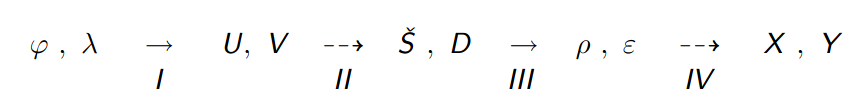
\includegraphics[width=1\textwidth]{FIG/schema}
\caption{Obecná schéma možného převodu elipsoidicých souřadníc do systému zobrazovacích souřadníc.}
\label{fig:schema}
\end{center}
\end{figure}


\begin{enumerate}
\item Blok \textbf{I} představuje konformní zobrazení elipsoidických souřadníc na kouli (například Gaussovým způsobem).
\item Blok \textbf{II} jsou zeměpisne sférické spuřadnice převedeny na kartografické souřadnice a to vzhledem k zvolenému kartografckému pólu.
\item  Blok \textbf{III} obsahuje konformní zobrazení kartografických souřadníc z koule na zvolenou zobrazovací plochu (kužel, válec, rovina).
\item Blok \textbf{IV} obsahuje výpočet pravouhlých souřadníc z polárních souřadníc.
\end{enumerate}

Meridiánová konvergence je úhel mezi zemským poledníkem a rovnoběžkou rovnoběžnou s osou Y (X - v závislosti na tom, jak je souřadnicový sýstém zobrazovací roviny definován). 

Speciálne pro stereografickou projekci, pokud by byla stereografická projekce v normálni poloze (na pólu) tak meridiánová konvergence se rovná přímo zeměpisné délce. Pokud stereografická projekce bude definováná v obecné poloze, postup odhadu meridánové konvergence by mohl být tento: 

\begin{itemize}
\item Zeměpisné souřadnice U, V pomocí nasledujících vztahů převedeme na kartografické souřadnice, s, d (platí pro převod na koulové ploše)
\begin{equation}
\sin{\left(s\right)} = \sin{\left(U_{k}\right)}\sin{\left(U\right)}+\cos{\left(U_{k}\right)}\cos{\left(U\right)}\cos{\left(\Delta V\right)}
\end{equation}
\begin{equation}
\sin{\left(d\right)}=\dfrac{\sin{\left(\Delta V\right)}\cos{\left(U\right)}}{\cos{\left(s\right)}}.
\end{equation}
\item Nasleduje výpočet souřadnice $\varepsilon$, například pomocí této zobrazovací rovnice
\begin{equation}
\varepsilon = nD,
\end{equation}
kde D je zeměpisná délka na kouli a n je konstanta zobrazení.
\item U vrcholu P sféfirckého trojuholníku se musí vypočítat vnitří úhel $\xi$
\begin{equation}
\sin{\left(\xi\right)} = \dfrac{\cos{\left(U_{k}\right)}\sin{\left(D\right)}}{\sin{\left(U\right)}}.
\end{equation}
\item Potom meridiánová konvergence se vypočte pomocí rovnice $C = \varepsilon - \xi$. Platí také přibližný vzorec
\begin{equation}
C = 0.008257 Y + 2.373\dfrac{Y}{X}\ [km],
\end{equation}
kde Y a X jsou pravouhlé souřadnice, přičemž X je obrazem základního poledníku a Y je kolmá na X.
\end{itemize}